\documentclass{beamer}

%\usepackage{multimedia}

% For more themes, color themes and font themes, see:
% http://deic.uab.es/~iblanes/beamer_gallery/index_by_theme.html
%
\mode<presentation>
{
  \usetheme{Madrid}       % or try default, Darmstadt, Warsaw, ...
  \usecolortheme{seahorse} % or try albatross, beaver, crane, ...
  \usefonttheme{serif}    % or try default, structurebold, ...
  \setbeamertemplate{navigation symbols}{}
  \setbeamertemplate{caption}[numbered]
} 

\usepackage{tikz}
\usetikzlibrary{decorations.markings,angles}
\usepackage{tikz-3dplot} 

\usepackage{amsmath}


\begin{document}

\begin{frame}{Different time behaviour}
\begin{figure}[H]
 \centering
 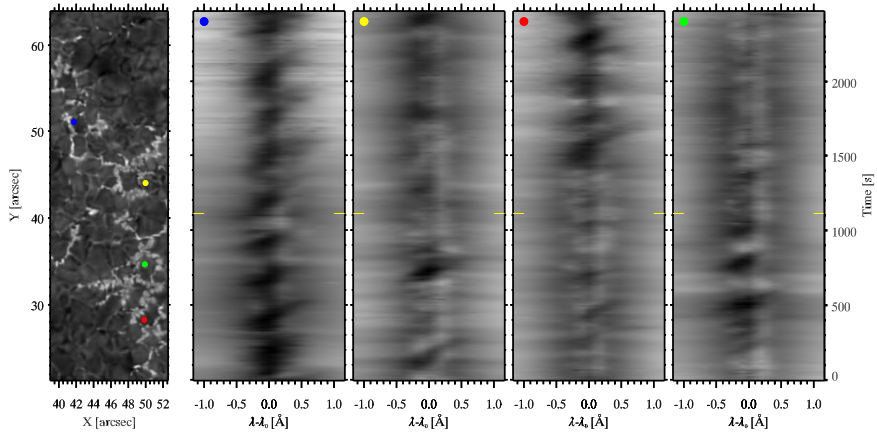
\includegraphics[scale=0.4]{im1.png}
\end{figure}

\end{frame}

\begin{frame}{Autocovariance timescale}
\begin{figure}[H]
 \centering
 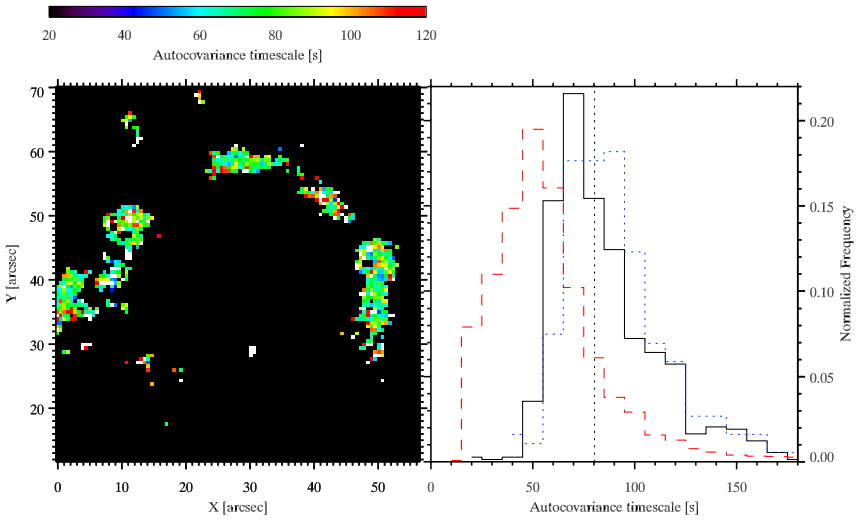
\includegraphics[scale=0.4]{im2.png}
\end{figure}

\end{frame}

\begin{frame}{Frames from Fig.2 animation movie}

%\movie[height = 0.6\textwidth, width = 0.8\textwidth, poster, showcontrols] {}{video.avi}

\begin{figure}[H]
 \centering
 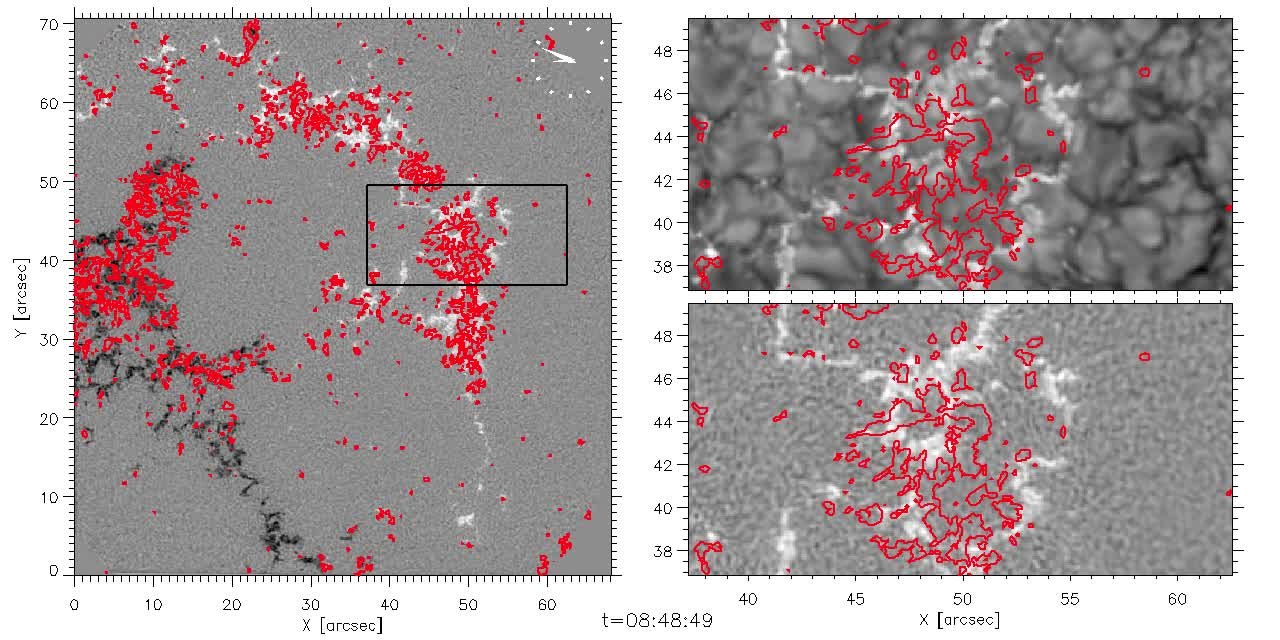
\includegraphics[scale=0.28]{output006.jpg}
\end{figure}

\end{frame}
\begin{frame}{Frames from Fig.2 animation movie}

\begin{figure}[H]
 \centering
 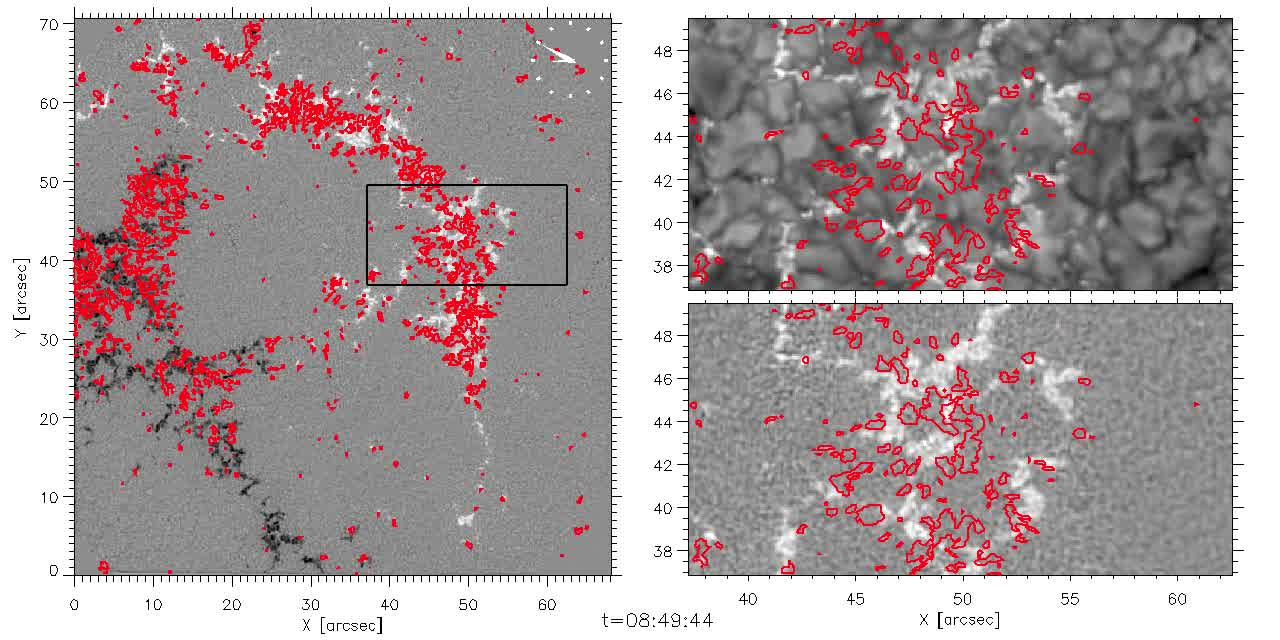
\includegraphics[scale=0.28]{output007.jpg}
\end{figure}

\end{frame}
\begin{frame}{Frames from Fig.2 animation movie}
\begin{figure}[H]
 \centering
 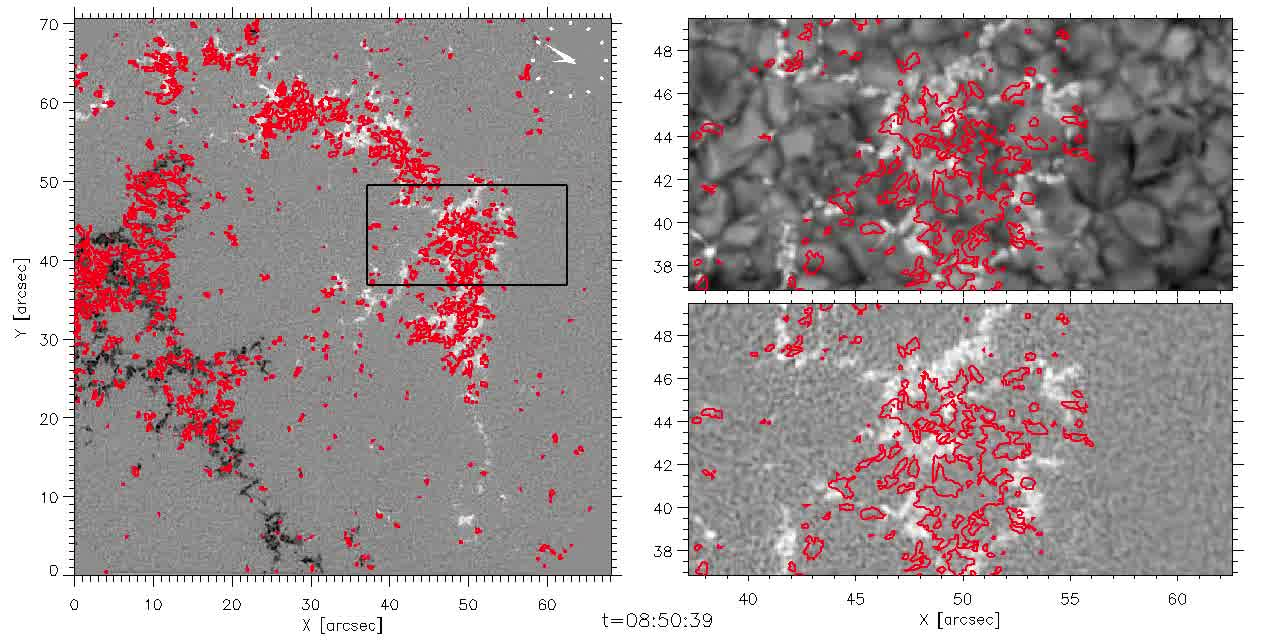
\includegraphics[scale=0.28]{output008.jpg}
\end{figure}

\end{frame}

\begin{frame}{Frames from Fig.2 animation movie}
\begin{figure}[H]
 \centering
 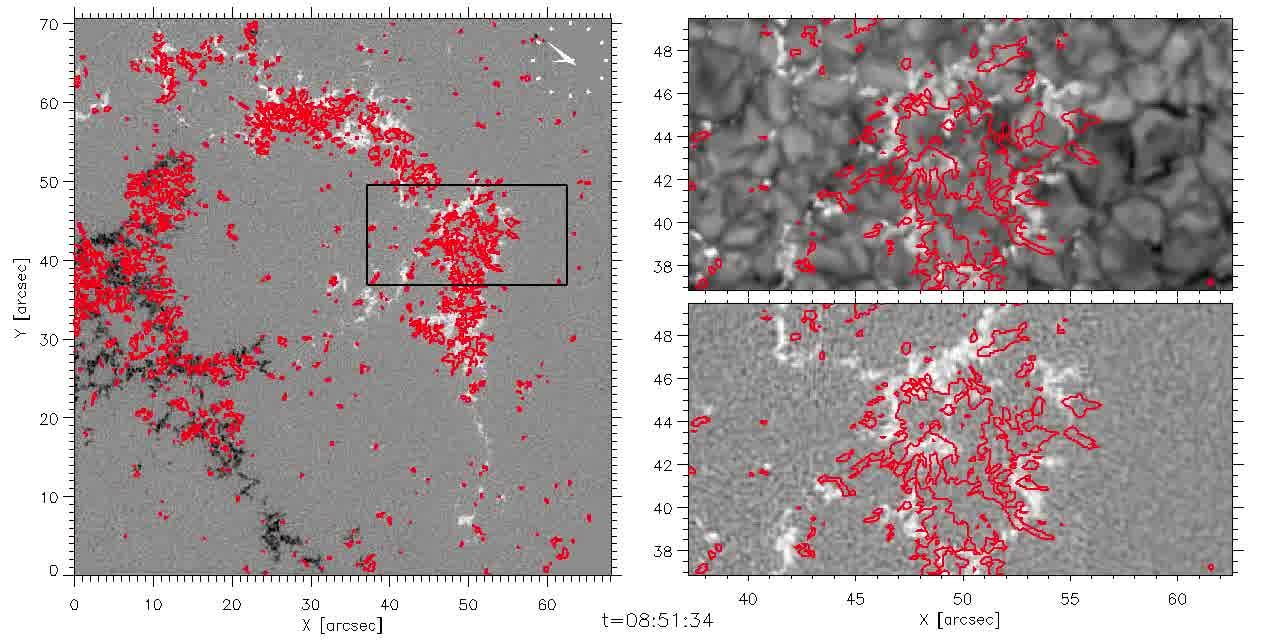
\includegraphics[scale=0.28]{output009.jpg}
\end{figure}

\end{frame}

\end{document}
